\chapter{Diseño del sistema}
\label{ch:diseno}
Tras haber realizado el análisis del sistema previamente, en este capítulo se desarrolla más en detalle las parte internas del sistema, como son las relacionadas con la arquitectura del sistema (\autoref{sec:arquitectura}), donde se define la manera en la que se relacionan y comunican las distintas partes que componen el sistema. 

También se define la manera en la que se almacenan los datos (\autoref{sec:modelo}) y como son las interfaces que componen el sistema (\autoref{sec:interfaz}) con las que interactúa el usuario. 

Además lo definido a continuación sienta la base para poder comenzar el desarrollo e implementación del sistema que se define en los siguientes capítulos, \autoref{ch:implementacion} y \autoref{ch:pruebas}.

\section{Arquitectura del Sistema}\label{sec:arquitectura}
El sistema que se desarrolla en este proyecto sigue un patrón de desarrollo bien definido, Modelo-Vista-Controlador, que nos permite separar de una manera clara las diferentes partes del sistema que hay que desarrollar. Esta arquitectura se compone de las siguientes partes:
\begin{itemize}
    \item \textbf{Modelo:} Parte encargada de la representación lógica de la información en el sistema, los mecanismos para acceder y almacenarla. Esta será la parte relacionada con la base de datos.
    \item \textbf{Vista:} Es la representación visual del sistema que se mostrará al usuario cuando utilice la aplicación.
    \item \textbf{Controlador:} Representa toda la lógica del sistema, tanto el procesamiento de las medidas como el tratamiento de las peticiones al servidor.
\end{itemize}

Esta separación en tres partes permite que se puedan desarrollar e implementar las 3 partes en paralelo, de manera que quede todo más modularizado y dado el caso se puedan modificar o remplazar sin problema. Como podría ser que quisiéramos cambiar la página web (vista) por otra diferente sin que haga falta modificar el modelo y controlador. 

Además, es ampliamente usado y se ha demostrado su eficacia en multitud de proyectos de software.
\pagebreak

En la \autoref{fig:mvc} se puede ver cuál es la relación entre las diferentes partes que lo componen, que son:
\begin{itemize}
    \item El usuario en primer lugar solicita al servidor que le mande la página web. También cuando visualice la web realizara solicitudes de servicios y contenidos que va visualizando.
    \item El controlador recibe las solicitudes del usuario y se comunica con la vista, para que mandar la parte visual del sistema al usuario y que puede realizar más solicitudes. Cuando necesita acceder a información o almacenarla se comunica con el modelo, para que se encargue este.
    \item El modelo almacena los datos y cuando se le solicita los manda o almacena.
    \item La vista envía al usuario la parte visual del sistema que le vaya diciendo el controlador que es el que se encarga de la parte lógica de la web.
\end{itemize}

\begin{figure}[H]
	\ffigbox[\FBwidth]
	{\caption{Diagrama Modelo-Vista-Controlador}
    \label{fig:mvc}}
	{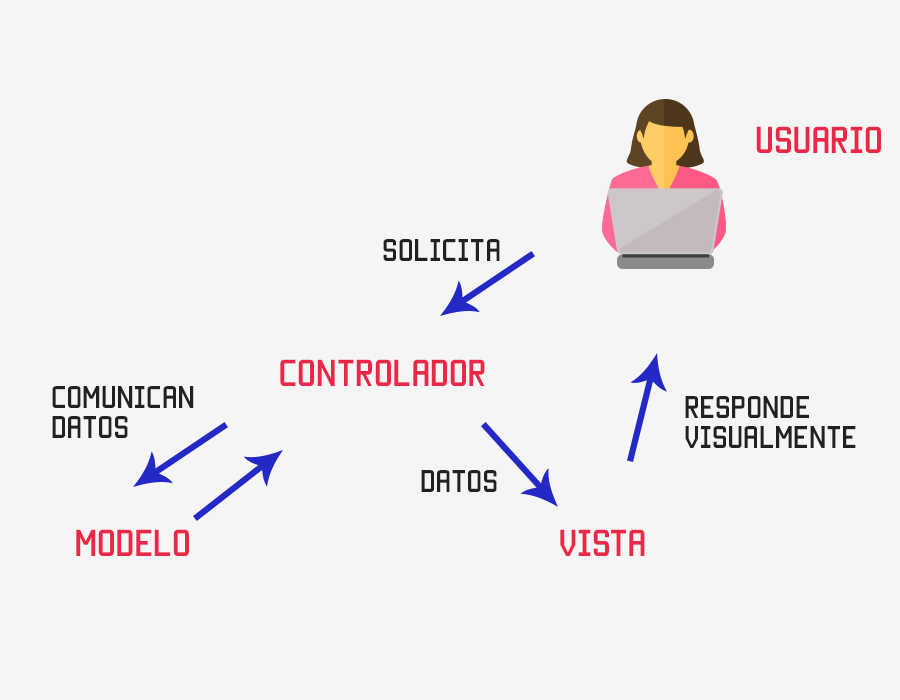
\includegraphics[scale=0.3]{mvc.jpg}}
\end{figure}

La manera en la que el usuario interactúa con el sistema será de Cliente-Servidor, lo que quiere decir que el usuario lo único que tendrá que hacer para utilizar el sistema será conectarse y acceder, será nuestro servidor el que tendrá todo el sistema y se encarga de responder todas las peticiones, gestionando los dispositivos, datos y web. 

En las siguientes secciones se define la parte de Modelo (\autoref{sec:modelo}) y Controlador (\autoref{sec:interfaz}).
\pagebreak

\section{Modelo de datos}\label{sec:modelo}
En este proyecto la base de datos es uno de los elementos más importantes que lo componen, no solo para permitir el acceso del personal autorizado a la aplicación, sino porque almacenará el histórico de las medidas tomadas en la sala.

La base de datos estará alojada en el servidor, donde podrá ser accedida por la aplicación más fácilmente para su visualización y consulta, además facilita que se puedan centralizar las medidas en un único lugar, para el caso de que se tuvieran múltiples dispositivos en un edificio y se deseara consultarlos desde un mismo lugar.

\subsection{Estructura de tablas de base de datos}
Las tablas que componen nuestra base de datos se describen a continuación.

Tabla de usuarios\dots
\begin{itemize}
    \item id
    \item estado...
\end{itemize}


Tabla de medidas\dots
\begin{itemize}
    \item dispositivo
    \item fecha
    \item temp...
\end{itemize}

\section{Interfaz de Usuario}\label{sec:interfaz}